\documentclass[a4wide,9pt,landscape]{article}
\usepackage[utf8]{inputenc}
\usepackage{url}
\usepackage{hyperref}
\usepackage{xcolor}
\usepackage{pgf,tikz}
\usepackage{amsmath}
\usepackage{amsthm}
\usepackage{amssymb}
\usepackage{tabularx}
%\usepackage{microtype}
%\usepackage{geometry}
\usepackage{titlesec}
\usepackage{fancyvrb}
\usepackage{relsize}
\usepackage{color,graphicx}
\usepackage{auto-pst-pdf}
\usepackage{pstricks, pstricks-add}
%\usepackage{picins}
\usepackage{scalerel}
\usepackage{booktabs}
\usepackage{multicol}
\usepackage{adgsignature}
%\usepackage{pdflscape}
%\usepackage{tikz,times}
%\usetikzlibrary{arrows,decorations.pathmorphing,backgrounds,fit,positioning,shapes.symbols,shapes.geometric,chains}


%\definecolor{ared}{rgb}{.647,.129,.149}
%\renewcommand\colorchapnum{\color{ared}}
%\renewcommand\colorchaptitle{\color{ared}}

% !TEX program = xelatex
% Ltex config: language=english

\hypersetup{
    colorlinks,
    linkcolor={red!50!black},
    citecolor={blue!50!black},
    urlcolor={blue!80!black}
}


%\newtheorem{definition}{Definition}
%\newtheorem{theorem}{Theorem}

\def\ll{\mbox{\begin{picture}(7,10)
\put(1,0){\line(1,0){5}}
\put(1,0){\line(0,1){5}}
\end{picture}
}}

\colorlet{almostwhite}{black!1}

\newcommand{\betweenSymbol}{\raisebox{0.004\textheight}{\ensuremath{\mathord{
\includegraphics[width=0.02\textwidth]{between_symbol.eps}}}}}
\newcommand{\betweenStrictSymbol}{\raisebox{0.002\textheight}{\ensuremath{\mathord{
\includegraphics[width=0.02\textwidth]{between_strict_symbol.eps}}}}}
\newcommand{\outSymbol}{\raisebox{0.002\textheight}{\ensuremath{\mathord{
\includegraphics[width=0.02\textwidth]{out_symbol.eps}}}}}
\newcommand{\midpointSymbol}{\raisebox{0.002\textheight}{\ensuremath{\mathord{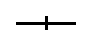
\includegraphics[width=0.02\textwidth]{midpoint_symbol.eps}}}}}
\newcommand{\falseLine}{\raisebox{0.004\textheight}{\ensuremath{\mathord{
\includegraphics[width=0.06\textwidth]{line.eps}}}}}
\newcommand{\trueLine}{\raisebox{0.002\textheight}{\ensuremath{\mathord{
\includegraphics[width=0.06\textwidth]{true_line.eps}}}}}
\newcommand{\perSymbol}{\raisebox{-0.2ex}{\ensuremath{\mathord{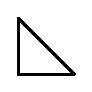
\includegraphics[height=0.7em]{per_symbol.eps}}}}}

\newcommand{\imp}{\Rightarrow}
\newcommand{\nb}{10\xspace}
\newcommand{\smallfigs}[2]{\centering
\scalebox{0.8}{\subfloat{#1}}
\qquad
\scalebox{0.8}{\subfloat{#2}}}

\newcommand{\myfrac}[3]{\substack{{\smaller[2] {#1}}\\ #2\\ {\smaller[2] {#3}}}}

%\newcommand{\bT}[3]{{#1} \betweenSymbol {#2} \betweenSymbol {#3}}
\DeclareMathOperator{\coll}{Col}
\newcommand{\col}[3]{\coll \, {#1} \, {#2} \, {#3}}
\newcommand{\out}[3]{{#1} \betweenStrictSymbol {#2} \outSymbol {#3}}
\newcommand{\midpoint}[3]{{#1} \midpointSymbol {#2} \midpointSymbol {#3}}
\newcommand{\per}[3]{\perSymbol \, {#1} \, {#2} \, {#3}}
\newcommand{\perpin}[3]{{#1} \mathbin{\underset{#3}{\perp}} {#2}}
\newcommand{\perpT}[2]{{#1} \mathbin{\perp} {#2}}
\newcommand{\indep}{\raisebox{0.2ex}{\scaleobj{0.9}{\rotatebox[origin=c]{90}{$\models$}}}}
\newcommand{\perpTwo}[3]{{#1} \mathbin{\underset{#3}{\indep}} {#2}}
\newcommand{\lineRefl}[4]{\mathsurround0pt {#1} \myfrac{{#3} \raisebox{0.002\textheight}{\scalebox{0.5}{$\text{\textbullet}$}} {\color{white} {#4}}}{\falseLine}{{\color{white} {#3}} \raisebox{0.002\textheight}{\scalebox{0.5}{$\text{\textbullet}$}} {#4}} {#2}}
\newcommand{\refl}[4]{\mathsurround0pt {#1} \myfrac{{#3} \raisebox{0.002\textheight}{\scalebox{0.5}{$\text{\textbullet}$}} {\color{white} {#4}}}{\trueLine}{{\color{white} {#3}} \raisebox{0.002\textheight}{\scalebox{0.5}{$\text{\textbullet}$}} {#4}} {#2}}
\newcommand{\tS}[4]{\mathsurround0pt {#1} \myfrac{{\color{white} {#3}} {#4}}{\trueLine}{{#3} {\color{white} {#4}}} {#2}}
%\newcommand{\tS}[4]{two-sides {#1} {#2} {#3} {#4}}
\newcommand{\oS}[4]{\mathsurround0pt {#1} \myfrac{\color{white} {#3} {#4}}{\trueLine}{{#3} {#4}} {#2}}
\DeclareMathOperator{\cpp}{Cp}
\newcommand{\cp}[4]{\cpp \, {#1} \,{ #2} \, {#3} \, {#4}}
\newcommand{\spara}[2]{{#1}\mathbin{\parallel_{s}} {#2}}
\newcommand{\para}[2]{{#1}\mathbin{\parallel} {#2}}
\newcommand{\perpBisect}[4]{\mathsurround0pt {#1} \myfrac{{#3} \raisebox{0.002\textheight}{\scalebox{0.5}{$\text{\textbullet}$}} {\color{white} {#4}}}{\trueLine_s}{{\color{white} {#3}} \raisebox{0.002\textheight}{\scalebox{0.5}{$\text{\textbullet}$}} {#4}} {#2}}
\newcommand{\bH}[3]{{#1} \betweenStrictSymbol {#2} \betweenStrictSymbol {#3}}

\newcommand{\angleT}[3]{{#1} \, {#2} \, {#3}}
\DeclareMathOperator{\congaa}{\mathbin{\widehat{=}}}
\newcommand{\conga}[6]{\angleT{#1}{#2}{#3} \congaa \angleT{#4}{#5}{#6}}
\DeclareMathOperator{\inangle}{\mathbin{\widehat{\in}}}
\newcommand{\inangleT}[4]{ {#1} \inangle \angleT{#2}{#3}{#4}}
\DeclareMathOperator{\leaa}{\mathbin{\widehat{\leq}}}
\DeclareMathOperator{\geaa}{\mathbin{\widehat{\geq}}}
\DeclareMathOperator{\gtaa}{\mathbin{\widehat{\gtq}}}
\DeclareMathOperator{\ltaa}{\mathbin{\widehat{<}}}
\newcommand{\lea}[6]{\angleT{#1}{#2}{#3} \leaa \angleT{#4}{#5}{#6}}
\newcommand{\lta}[6]{\angleT{#1}{#2}{#3} \ltaa \angleT{#4}{#5}{#6}}
\newcommand{\gea}[6]{\angleT{#1}{#2}{#3} \leaa \angleT{#4}{#5}{#6}}
\newcommand{\gta}[6]{\angleT{#1}{#2}{#3} \ltaa \angleT{#4}{#5}{#6}}
\DeclareMathOperator{\acutea}{acute}
\newcommand{\acuteT}[3]{\acutea \, \angleT{#1}{#2}{#3}}
\DeclareMathOperator{\sumaa}{\mathbin{\widehat{+}}}
\DeclareMathOperator{\eqaa}{\mathbin{\widehat{=}}}
\newcommand{\suma}[9]{\angleT{#1}{#2}{#3} \sumaa \angleT{#4}{#5}{#6} \eqaa \angleT{#7}{#8}{#9}}
\DeclareMathOperator{\sams}{Sams}
\newcommand{\samsT}[6]{\sams (\angleT{#1}{#2}{#3}, \, \angleT{#4}{#5}{#6})}
\DeclareMathOperator{\trisum}{\mathcal{S}}
\newcommand{\trisuma}[6]{\trisum(\bigtriangleup{#1}{#2}{#3}) \eqaa \angleT{#4}{#5}{#6}}

\newcommand{\jn}[1]{\textcolor{blue}{JN: #1}}


\DefineVerbatimEnvironment
{CoqVerbatim}{Verbatim}
{frame=lines, fontsize=\small}

\psset{algebraic=true,dotstyle=o,dotsize=3pt 0,linewidth=0.8pt,arrowsize=3pt 2,arrowinset=0.25}

\newcommand{\hi}[1]{\textcolor{red}{#1}}

\title{A standard signature for the ADGlib}
\author{ADG Foundation}
\date{\today}


\begin{document}

\maketitle

\begin{abstract}
  This document describes the signature of the ADGlib library.
  
  The signature is a collection of predicates and functions for the
  manipulation of geometric objects.
  
  The objective is to facilitate the communication between different
  tools manipulating geometric statements. 

  The {\em core} predicate symbols has to be supported by any
  translation and here they are given in bold face.

  The axiom system used may assume if the geometry is planar,
  Euclidean, etc.
  
\end{abstract}




\section{General conventions}


\newpage


\pagestyle{empty}


\noindent\hspace{-75mm}
\begin{tabularx}{270mm}{>{\ttfamily}llXX}
\toprule
\multicolumn{4}{l}{\Huge Points-only; predicate symbols (1/4)} \\ \midrule
ADGLib & 
\LaTeX{} notation & 
Intuitive meaning & 
Definition \\ \midrule
%-------------------------------------------------------------------
{\bf between(A,B,C)} & 
& 
points $A$, $B$ and $C$ are collinear and $B$ is strictly between $A$ and $C$ \\
%-------------------------------------------------------------------
betweenNonStrict(A,B,C) &  
$\bT{A}{B}{C}$ & 
points $A$, $B$ and $C$ are collinear and $B$ is between $A$ and $C$, it can be the case the $A=B$ or $B=C$. & 
\\
%-------------------------------------------------------------------
between4(A,B,C,D) & 
& 
points $A$, $B$ $C$ and $D$ are collinear distinct and in this order. \\
%-------------------------------------------------------------------
centroid(H,A,B,C) & 
& 
$H$ is the centroid/gravity center of triangle $ABC$. \\
%-------------------------------------------------------------------
circumcenter(G,A,B,C) & 
& 
$G$ is the circum-center of the three points $ABC$. \\
%-------------------------------------------------------------------
{\bf collinear(A,B,C)} & 
$\col{A}{B}{C}$ & 
points $A$, $B$ and $C$ are collinear & 
$ \bT{A}{B}{C} \lor \bT{B}{A}{C} \lor \bT{A}{C}{B} $ \\
%-------------------------------------------------------------------
%collinearStrict(A,B,C) & 
%& 
%points $A$, $B$ and $C$ are distinct collinear points. \\
%-------------------------------------------------------------------
{\bf concyclic(A,B,C,D)} &  
& 
$A$, $B$, $C$ and $D$ belong to the same circle & 
$Coplanar A B C D \land \exists O\; \congT{OA}{OB} \land \congT{OA}{OC}  \land \congT{OA}{OD} $ \\
%-------------------------------------------------------------------
\addlinespace
%-------------------------------------------------------------------
{\bf congruent(A,B,C,D)} & 
$\congT{AB}{CD}$ & 
the segments $AB$ and $CD$ are congruent (intuitively in the sense that they have 
same length, but length measure is not assumed to exist) \\
%-------------------------------------------------------------------
{\bf congruentAngles(A,B,C,D,E,F)} & 
$ \conga{A}{B}{C}{D}{E}{F} $ & 
the angles $\angle{ABC}$ and $\angle{DEF}$ are congruent & 
$ A \neq B \land C \neq B \land D \neq E \land F \neq E \land $ \\
& & & $ \exists A', \exists C', \exists D', \exists F',  \bT{B}{A}{A'} \land \congT {AA'}{ED} \land $ \\
& & & $ \bT {B}{C}{C'} \land \congT {CC'}{EF} \land  \bT {E}{D}{D'} \land \congT {DD'}{BA} \land $\\
& & & $ \bT {E}{F}{F'} \land \congT {FF'}{BC} \land  \congT {A'C'}{D'F'} $  \\
%-------------------------------------------------------------------
congruentCircles(O,P,O',P') & 
& 
the two circles are congruent. \\
%-------------------------------------------------------------------
{\bf congruentTriangles(A,B,C,A',B',C')} & 
& 
$ABC$ is congruent to $A'B'C'$ & 
$ \congT{AB}{A'B'} \land \congT{AC}{A'C'} \land \congT{BC}{B'C'} $ \\
%-------------------------------------------------------------------
congruentRectangles(A,B,C,D,A',B',C',D') & 
& 
$ABCD$  and $A'B'C'D'$ are congruent rectangles & 
$ \congT{AB}{A'B'} \land \congT{BC}{B'C'} \land Rectangle(A,B,C,D) \land Rectangle(A',B',C',D') $ \\
%----------------------------------------------------------------
diameter(A,B,O,P) & 
& 
$AB$ is a diameter of the circle of center $O$ going through $P$. \\
%-------------------------------------------------------------------
equilateral(A,B,C) & 
& 
$ABC$ is an equilateral triangle & 
$\congT{AB}{BC} \land \congT{BC}{CA}$\\
%-------------------------------------------------------------------
equilateralNdg(A,B,C) & 
& 
$ABC$ is an equilateral triangle and the points are distinct and hence not collinear & 
$equilateral A B C \land A \neq B$ \\
%-------------------------------------------------------------------
harmonic(A,B,C,D) & 
& 
Points $A$, $B$, $C$, $D$ are on the same line and $AC/CB=DA/DB$. \\
%-------------------------------------------------------------------
incenterNdg(G,A,B,C) & 
& 
$G$ is the in-center of ndg triangle $ABC$. \\
%-------------------------------------------------------------------
\bottomrule
\end{tabularx}

\newpage

\noindent\hspace{-75mm}
\begin{tabularx}{270mm}{>{\ttfamily}llXX}
\toprule
\multicolumn{4}{l}{\Huge Points-only; predicate symbols (2/4)} \\ \midrule
ADGLib & 
\LaTeX{} notation & 
Intuitive meaning & 
Definition \\ \midrule
%-------------------------------------------------------------------
insideCircleStrict(C,O,P) & 
& 
$C$ is strictly inside or on circle (or sphere) of center $O$ going through $P$.\\
%-------------------------------------------------------------------
insideCircle(C,O,P) & 
& 
$C$ is inside the circle (or sphere) of center $O$ going through $P$.\\
%-------------------------------------------------------------------
insideAngle(P,A,B,C) & 
$ \inangleT{P}{A}{B}{C} $ & 
the point $P$ is inside the angle $\angle{ABC}$ & 
$A \neq B \land C \neq B \land P \neq B \land \exists X, \bT{A}{X}{C} \land$ \\
 & & & $ (X = B \lor \out{B}{X}{P}) $ \\
%-------------------------------------------------------------------
{\bf intersectionLineLine(X,A,B,C,D)} & &
$X$ is the intersection of lines $AB$ and $CD$ \\
%-------------------------------------------------------------------
intersectionLineSegment(X,A,B,C,D) & &
$X$ is the intersection of line $AB$ and segment $CD$ \\
%-------------------------------------------------------------------
{\bf intersectionLineCircle(X,Y,A,B,O,P)} & &
$X$ and $Y$ are the intersections of line $AB$ and circle $OP$ \\
%-------------------------------------------------------------------
intersectionSegmentSegment(X,A,B,C,D) & &
$X$ is the intersection of segments $AB$ and $CD$ \\
%-------------------------------------------------------------------
{\bf intersectionCircleCircle(X,Y,O,P,O',P')} & 
& 
$X$ and $Y$ are the intersections of circles $OP$ and $O'P'$. \\
%-------------------------------------------------------------------
isosceles(A,B,C) & 
& 
$ABC$ is an isosceles triangle in $B$, points may be equal. & 
$\congT{AB}{BC}$ \\
%-------------------------------------------------------------------
isoscelesNdg(A,B,C) & 
& 
$ABC$ is an isosceles triangle in $B$, points are not collinear. & 
$\congT{AB}{BC} \land \lnot \col{A}{B}{C} $  \\
%-------------------------------------------------------------------
kite(A,B,C,D) & 
& 
$ABCD$ is a kite & \\
%-------------------------------------------------------------------
lambert(A,B,C,D) & 
& 
$ABCD$ is a quadrilateral with three right angles. In hyperbolic geometry the fourth 
angle is acute, in Euclidean geometry it is a right angle. & 
$A\neq B \land B \neq C \land C \neq D \land A \neq D \land \per{B}{A}{D} \land \per{A}{D}{C} \land \per{A}{B}{C} $ \\
%-------------------------------------------------------------------
{\bf midpoint(M,A,B)} & 
$\midpoint{A}{M}{B}$ & 
$M$ is the midpoint of segment $AB$ & 
$\bT{A}{M}{B} \land \congT{A M}{B M} $ \\
%-------------------------------------------------------------------
{\bf onAngleBisector(P,A,O,B)} &  
& 
$P$ belongs to the bisector of angle $AOB$ & 
$P \neq O \land \angle{AOP}$ and $\angle{POB}$ are congruent \\
%-------------------------------------------------------------------
{\bf onCircle(C,O,P)} & 
& 
$C$ is on circle (or sphere) of center $O$ going through $P$. \\
%-------------------------------------------------------------------
{\bf onLine(P,A,B)} & 
& 
points $P$ is on line $AB$ ($A\neq B$). \\
%-------------------------------------------------------------------
\addlinespace
{\bf onParallel(P,B,C,D)} & 
 & 
$P$ is on the parallel to line $CD$ through $B$ & 
$ \para{A B}{C D} \land C \neq D $ \\
%-------------------------------------------------------------------
\addlinespace
{\bf onPerpendicular(P,B,C,D)} & 
 & 
$P$ is on the perpendicular to line $CD$ through $B$ & 
$ \perp{A B}{C D} \land C \neq D $ \\

%-------------------------------------------------------------------
{\bf onPerpendicularBisector(P,A,B)} &  
& 
$P$ belongs to the perpendicular bisector of segment $AB$ & 
$P \neq midpoint(A,B)$ and $\congT{PA}{PB}$ \\
%-------------------------------------------------------------------
{\bf onRay(O,A,B)} & 
$\out{O}{A}{B}$ & 
$B$ belongs to the half line $OA$ & $ O \neq A \land O  \neq B \land (\bT{O}{A}{B} \lor \bT{O}{B}{A}) $ \\
%-------------------------------------------------------------------
\bottomrule
\end{tabularx}

\newpage

\noindent\hspace{-75mm}
\begin{tabularx}{270mm}{>{\ttfamily}llXX}
\toprule
\multicolumn{4}{l}{\Huge Points-only; predicate symbols (3/4)} \\ \midrule
ADGLib & 
\LaTeX{} notation & 
Intuitive meaning & 
Definition \\ \midrule
%-------------------------------------------------------------------
{\bf oppositeSides(A,B,P,Q)} & 
$\tS{A}{B}{P}{Q}$ & 
$P$ and $Q$ are on different sides of line $AB$ & 
$ \lnot \col{P}{A}{B} \land \lnot \col{Q}{A}{B} \land \exists T, \col{T}{A}{B} \land \bT{P}{T}{Q} $ \\
%-------------------------------------------------------------------
outsideCircle(C,O,P) & 
& 
$C$ is on or outside the circle (or sphere) of center $O$ going through $P$.\\
%-------------------------------------------------------------------
outsideCircleStrict(C,O,P) & 
& 
$C$ is strictly outside the circle (or sphere) of center $O$ going through $P$.\\
%-------------------------------------------------------------------
{\bf meetLineLine(A,B,C,D)} & 
& 
The lines $AB$ and $CD$ intersect. \\
%-------------------------------------------------------------------
meetLineSegment(A,B,C,D) & 
& 
The line $AB$ and segment $CD$ intersect. \\
%-------------------------------------------------------------------
meetSegmentSegment(A,B,C,D) & 
& 
The segment $AB$ and segment $CD$ intersect. \\
%-------------------------------------------------------------------
orthocenter(H,A,B,C) & 
& 
$H$ is the orthocenter of triangle $ABC$. \\
%-------------------------------------------------------------------
{\bf perpendicular(A,B,C,D)} & 
$\perpT{A B}{C D} $ & 
line $AB$ is perpendicular to line $CD$ ($A\neq B$ and $C\neq D$) & 
$ \exists P, \perpin{AB}{CD}{P} $ \\
%-------------------------------------------------------------------
perpendicularAt(P,A,B,C,D) & 
$\perpin{A B}{C D}{P}$ & 
$AB \bot CD$ and $P$ is the intersection of $AB$ and $CD$ & 
$A \neq B \; \land \; C \neq D \; \land \; \col {P} {A} {B} \; \land \; \col {P} {C} {D} \; \land \; 
(\forall U \, V, \col {U} {A} {B} \imp \col {V} {C} {D} \imp \per{U}{P}{V})$ \\
%-------------------------------------------------------------------
\addlinespace
perpendicular2(A,B,C,D,P) & 
$\perpTwo{A B}{C D}{P}$ & 
the line $AB$ and $CD$ have a common perpendicular through $P$ & 
$ \exists X, \exists Y, \col{P}{X}{Y} \land \perpT{XY}{AB} \land \perpT{XY}{CD} $ \\
%-------------------------------------------------------------------
\addlinespace
{\bf parallel(A,B,C,D)} & 
$ \para{A B}{C D} $ & 
line $AB$ is parallel to line $CD$ & 
$ \spara{A B}{C D} \lor (A \neq B \land C \neq D \land \col{A}{C}{D} \land \col{B}{C}{D}) $ \\
%-------------------------------------------------------------------
\addlinespace
parallelNonStrict(A,B,C,D) & 
 & 
line $AB$ is parallel to line $CD$ or $A=B$ or $C=D$ & 
$ \para{A B}{C D} \lor (A=B \lor C=D) $ \\
%-------------------------------------------------------------------
parallelNonReflexive(A,B,C,D) & 
$\spara{A B}{C D} $ & 
line $AB$ is parallel to line $CD$ and $AB \neq CD$ & 
$A \neq B \land C \neq D \land \cp{A}{B}{C}{D} \land \lnot \exists X, \col{X}{A}{B} \land \col{X}{C}{D} $ \\
%-------------------------------------------------------------------
\addlinespace
verticalAngles(A,B,C,D,E,F) & 
 & 
$ABC$ and $DEF$ are vertical angles & 
$ B=E \land \bH{A}{B}{D} \land \bH{C}{B}{F} $ \\
%-------------------------------------------------------------------
parallelogram(A,B,C,D) & 
& 
$ABCD$ is a parallelogram, this includes a flat case defined as diagonals intersect in their midpoint & 
$Parallelogram\_strict \, A \, B \, A' \, B' \; \lor \; Parallelogram\_flat \, A \, B \, A' \, B'$ \\
%-------------------------------------------------------------------
parallelogramNdg(A,B,C,D) & 
& 
$ABCD$ is a parallelogram. The points are not collinear & 
$\oS {A} {A'} {B} {B'} \; \land \; AB \parallel A'B' \; \land \; \congT{AB}{A'B}'$ \\
%-------------------------------------------------------------------
parallelogramFlat(A,B,C,D) & 
& 
$ABCD$ is a flat parallelogram &
$ \col {A} {B} {A'} \; \land \; \col {A} {B} {B'} \; \land \congT {AB} {A'B}' \; \land \; \congT {AB'} {A'B} \; \land \; (A \neq A' \; \lor \; B \neq B') $ \\
%-------------------------------------------------------------------
\bottomrule
\end{tabularx}

\newpage

\noindent\hspace{-75mm}
\begin{tabularx}{270mm}{>{\ttfamily}llXX}
\toprule
\multicolumn{4}{l}{\Huge Points-only; predicate symbols (4/4)} \\ \midrule
ADGLib & 
\LaTeX{} notation & 
Intuitive meaning & 
Definition \\ \midrule
%-------------------------------------------------------------------
{\bf perpendicularBisector(P,Q,A,B)} & 
& 
$PQ$ is the perpendicular bisector of segment $AB$ &
$ ReflectL\,A\,B\,P\,Q \land A \neq B$ \\
%-------------------------------------------------------------------
quadrilateral(A,B,C,D) & & \\
%-------------------------------------------------------------------
quadrilateralNonCrossed(A,B,C,D) & & \\
%-------------------------------------------------------------------
rectangle(A,B,C,D) & 
& 
$ABCD$ is a rectangle (all points are distinct) & \\
%-------------------------------------------------------------------
reflectionStrict(P',P,A,B) & 
& 
$P'$ is the image of $P$ by reflection on line $AB$ & 
$(\exists X\; \midpoint{X}{P}{P'} \land \col{A}{B}{X}) \land (\perpT{AB}{PP'} \lor P=P')$ \\
%-------------------------------------------------------------------
{\bf reflection(P',P,A,B)} & 
& 
$P'$ is the image of $P$ by reflection on line $AB$ if $A\neq B$ and $P'$ is the image of $P$ by the reflection on point $A$ if $A=B$  & 
$(A\neq B \land ReflectL\,P'\,P\,A\, B) \lor (A=B \land \midpoint{A}{P}{P'})$ \\
%-------------------------------------------------------------------
regularPentagon(A,B,C,D,E) & & \\
%-------------------------------------------------------------------
regularHexagon(A,B,C,D,E,F) & & \\
%-------------------------------------------------------------------
rhombus(A,B,C,D) & 
& 
$ABCD$ is a rhombus & \\
%-------------------------------------------------------------------
rightAngle(A,B,C) & 
$ \per{A}{B}{C} $ & 
the triangle $ABC$ is a right triangle in $B$ & 
$\exists C', \midpoint{C}{B}{C'} \land \congT{A C}{A C'} $ \\
%-------------------------------------------------------------------
saccheri(A,B,C,D) & 
& 
$ABCD$ is a quadrilateral with two equal sides perpendicular to the base. In Euclidean geometry it is a rectangle. & 
$\per{B}{A}{D} \land \per{A}{D}{C} \land \congT{AB}{CD} \land \oS{A}{D}{B}{C}$ \\
%-------------------------------------------------------------------
{\bf sameSide(A,B,X,Y)} & 
$\oS {A}{B}{X}{Y}$ & 
$X$ and $Y$ are on the same side of line $AB$ & 
$ \exists Z, \tS{A}{B}{X}{Z} \land \tS{A}{B}{Y}{Z}$ \\
%-------------------------------------------------------------------
{\bf similarTriangles(A,B,C,A',B',C')} & 
& 
$ABC$ is similar to $A'B'C'$ & 
$\conga{A}{B}{C}{A'}{B'}{C'} \land \conga{B}{C}{A}{B'}{C'}{A'} \land \conga{C}{A}{B}{C'}{A'}{B'}$ \\
%-------------------------------------------------------------------
square(A,B,C,D) & 
& 
$ABCD$ is a square (all points are distinct) \\
%-------------------------------------------------------------------
\addlinespace
symmetric(P',P,I) & 
& 
$P'$ is the symmetric of $P$ wrt $I$ \\
%-------------------------------------------------------------------
trapezoid(A,B,C,D) & 
& 
$ABCD$ is a trapezoid: $AB$ is parallel to $CD$ &\\
%-------------------------------------------------------------------
trapezoidRight(A,B,C,D) & 
& 
$ABCD$ is a trapezium with a right angle in $A$. \\ 
%-------------------------------------------------------------------
trapezoidIsosceles(A,B,C,D) & 
& 
$ABCD$ is a trapezoid with congruent non necessary parallel sides: $AB$ is parallel to $CD$ and $\congT{BC}{DA}$\\
%-------------------------------------------------------------------
triangle(A,B,C) & 
& $A$, $B$, $C$ are non-collinear  
\\
\bottomrule
\end{tabularx}

\newpage

% ******************************************************************
% ******************************************************************
% ******************************************************************

\noindent\hspace{-75mm}
\begin{tabularx}{270mm}{>{\ttfamily}llXX}
\toprule
\multicolumn{4}{l}{\Huge Points-only; predicate symbols on comparison of segments and angles} \\ \midrule
ADGLib & 
\LaTeX{} notation & 
Intuitive meaning & 
Definition \\ \midrule
%-------------------------------------------------------------------
lessEqual(A,B,C,D) & 
$ AB \leq CD $ & the length $AB$ is smaller or equal to length $CD$ & 
$ \exists E, \bT{C}{Y}{D} \land \congT {AB}{CE} $ \\
%-------------------------------------------------------------------
lessThan(A,B,C,D) & 
$ AB < CD $ & 
the length $AB$ is smaller to length $CD$ & 
$ AB \leq CD \land \lnot \congT {AB}{CD} $ \\
%-------------------------------------------------------------------
greaterEqual(A,B,C,D) & 
$ AB \ge CD$ & 
the length $AB$ is greater or equal to length $CD$ & 
$ CD \leq AB $ \\
%-------------------------------------------------------------------
greaterThan(A,B,C,D) & 
$ AB > CD $ & 
the length $AB$ is greater than length $CD$ & 
$ CD < AB $ \\
%-------------------------------------------------------------------
\addlinespace
%-------------------------------------------------------------------
lessEqualAngles(A,B,C,D,E,F) & 
$ \lea{A}{B}{C}{D}{E}{F} $ & 
the angle $\angle{ABC}$ is smaller or equal than angle $\angle{DEF}$ & 
$ \exists P, \inangleT{P}{D}{E}{F} \land \conga{A}{B}{C}{D}{E}{P} $ \\
%-------------------------------------------------------------------
lessThanAngles(A,B,C,D,E,F) & 
$ \lta{A}{B}{C}{D}{E}{F} $ & 
the angle $\angle{ABC}$ is smaller than angle $\angle{DEF}$ & 
$ \lea{A}{B}{C}{D}{E}{F} \land \lnot \conga{A}{B}{C}{D}{E}{F}  $ \\
%-------------------------------------------------------------------
greaterThanAngles(A,B,C,D,E,F) & 
$\gta{A}{B}{C}{D}{E}{F}$ & 
the angle $\angle{ABC}$ is greater than angle $\angle{DEF}$ & 
$ \lta{D}{E}{F}{A}{B}{C} $\\
%-------------------------------------------------------------------
greaterEqualAngles(A,B,C,D,E,F) & 
$\gea{A}{B}{C}{D}{E}{F}$ & 
the angle $\angle{ABC}$ is greater than angle $\angle{DEF}$ & 
$ \lea{D}{E}{F}{A}{B}{C} $\\
%-------------------------------------------------------------------
acute(A,B,C) & 
& 
$\angle{ABC}$ is an acute angle (strictly) & 
$ \exists A', \exists B', \exists C', \per{A'}{B'}{C'} \land \lta{A}{B}{C}{A'}{B'}{C'} $ \\
%-------------------------------------------------------------------
obtuse(A,B,C) & 
& 
$\angle{ABC}$ is an obtuse angle (strictly) & 
$ \exists A', \exists B', \exists C', \per{A'}{B'}{C'} \land \lta{A'}{B'}{C'}{A}{B}{C} $\\
%-------------------------------------------------------------------
acuteTriangle(A,B,C) & 
& 
$ABC$ is a triangle with three acute angles. \\
%-------------------------------------------------------------------
obtuseTriangle(A,B,C) & 
& 
$ABC$ is a triangle with one obtuse angle. \\
%-------------------------------------------------------------------
supplementary(A,B,C,D,E,F) & 
& 
the angles $\angle{ABC}$ and $\angle{DEF}$ are supplementary & 
$ A \neq B \land \exists A', \bT{A}{B}{A'} \land \conga{D}{E}{F}{C}{B}{A'} $\\
%-------------------------------------------------------------------
sumSegments(A,B,C,D,E,F) & 
& 
$EF$ is congruent to the sum of $AB$ and $CD$ \\ 
%-------------------------------------------------------------------
sumAngles(A,B,C,D,E,F,G,H,I) & 
$\suma{A}{B}{C}{D}{E}{F}{G}{H}{I}$ & 
The sum of angles $\angle{ABC}$ and $\angle{DEF}$ is congruent to $\angle{GHI}$ & 
$ \exists\,J\; \conga{C}{B}{J}{D}{E}{F} \land \lnot \oS{B}{C}{A}{J} \land \cp{A}{B}{C}{J} \land \conga{A}{B}{J}{G}{H}{I} $ \\
%-------------------------------------------------------------------
sumAnglesLessThanStraightAngle(A,B,C,D,E,F) & 
& 
The sum of the angles $\angle{ABC}$ and $\angle{DEF}$ is smaller than the straight angle. & 
$ A\neq B \land (Out E D F \lor \lnot \bT{A}{B}{C}) \land
  \exists\,J\; \conga{C}{B}{J}{D}{E}{F} \land \lnot \oS{B}{C}{A}{J} \land \lnot \tS{A}{B}{C}{J} \land \cp{A}{B}{C}{J} $ \\
%-------------------------------------------------------------------
sumAnglesTriangleCongruent(A,B,C,D,E,F) & 
$\trisuma{A}{B}{C}{D}{E}{F}$ & 
The sum of the angles of the triangle $ABC$ is congruent to the angle $\angle{D}{E}{F}$ & 
$\exists G\,H\,I\; SumA\; A\, B\, C\, B\, C\, A\, G\, H\, I \land SumA\; G\, H \,I\, C\, A\, B\, D\, E\, F $ \\
%-------------------------------------------------------------------
sumAnglesDefect(A,B,C,D,E,F) & 
& 
The difference between the sum of angles of ABC and a straight angle. \\
%-------------------------------------------------------------------
\addlinespace
%-------------------------------------------------------------------
isoscelesRight(A,B,C) & 
& 
$ABC$ is a right and isosceles triangle in $B$. \\
%-------------------------------------------------------------------
\addlinespace
\bottomrule
\end{tabularx}

\newpage

% ******************************************************************
% ******************************************************************
% ******************************************************************

\noindent\hspace{-75mm}
\begin{tabularx}{270mm}{>{\ttfamily}llXX}
\toprule
\multicolumn{4}{l}{\Huge Points-only; predicates on coordinates} \\ \midrule
ADGLib & 
\LaTeX{} notation & 
Intuitive meaning & 
Definition \\ \midrule
\addlinespace
sum(O,E,E',A,B,C) & & In the grid $OEE'$ the sum of A and B is C \\
product(O,E,E',A,B,C) & & In the grid $OEE'$ the product of A and B is C \\
opposite(O,E,E',A,B) & & In the grid $OEE'$ the opposite of A is B \\
difference(O,E,E',A,B,C) & & In the grid $OEE'$ the difference between A and B is C \\
LtP(O,E,E',A,B) & & In the gird $OEE'$, A and B are positive \\
\bottomrule
\end{tabularx}

\newpage

% ******************************************************************
% ******************************************************************
% ******************************************************************

\noindent\hspace{-75mm}
\begin{tabularx}{270mm}{>{\ttfamily}llXX}
\toprule
\multicolumn{4}{l}{\Huge Points-only; deterministic function symbols} \\ \midrule
ADGLib & 
\LaTeX{} notation & 
Intuitive meaning & 
Definition \\ \midrule
%-------------------------------------------------------------------
funAnotherPoint(A,B) & 
&
a point on line $AB$ different from $A$ and $B$ \\
%-------------------------------------------------------------------
funCentroid(A,B,C) & 
&
the centroid (gravity center) of triangle $ABC$ \\
%-------------------------------------------------------------------
funCircumcenter(A,B,C) & 
&
the circumcenter of triangle $ABC$ \\
%-------------------------------------------------------------------
funEquilateral\_from(A,B) & 
&
A point $C$ such that $ABC$ is an equilateral triangle. \\
%-------------------------------------------------------------------
funEquilateral\_from\_on\_side(A,B,P) & 
&
A point $C$ such that $ABC$ is an equilateral triangle, and $C$ and $P$ are on the same side of line $AB$. \\
%-------------------------------------------------------------------
funExtend(A,B) & &
a point on half-line $AB$ such that $B$ is between $A$ and the new point. \\
%-------------------------------------------------------------------
funExtendDistance(A,B,P,Q) & &
a point $N$ on half-line $AB$ such that $B$ is between $A$ and $N$ and $BN$ is congruent to $PQ$. This corresponds to a compass. \\
%-------------------------------------------------------------------
funFoot(A,B,P) & 
&
the foot of the perpendicular to $AB$ through $P$ \\
%-------------------------------------------------------------------
funIncenter(A,B,C) & 
&
the incenter of triangle $ABC$ \\
%-------------------------------------------------------------------
funIntersectionLineLine(A,B,C,D) & 
&
the intersection of lines AB and CD (assuming they do interesect ? ) \jn{undefined if they do not intersect ?}\\
%-------------------------------------------------------------------
funIntersectionLineSegment(A,B,C,D) & 
&
intersection of line $AB$ and segment $CD$. \\
%-------------------------------------------------------------------
funIntersectionLineCircle(A,B,O,P) & 
&
intersection of line $AB$ and circle of center $O$ going through $P$. \jn{what to do when there are two intersections ?} \\
%-------------------------------------------------------------------
funIntersectionSegment\_circle(A,B,O,P) & 
&
intersection of segment $AB$ and circle of center $O$ going through $P$. \jn{what to do when there are two intersections ?} \\
%-------------------------------------------------------------------
fun\_intersection\_segment\_segment(A,B,C,D) & 
&
intersection of segment $AB$ and segment $CD$. \\
%-------------------------------------------------------------------
funIsoscelesFrom(A,B) & 
&
A point $C$ such that $ABC$ is an isosceles triangle in $C$. \\
%-------------------------------------------------------------------
funIsoscelesFromOnSide(A,B,P) & 
&
A point $C$ such that $ABC$ is an isosceles triangle in $C$ and $C$ 
is on the same side of line $AB$ as $P$. \\
%-------------------------------------------------------------------
funMidpoint(A,B) & 
&
the midpoint of segment $AB$ \\
%-------------------------------------------------------------------
funOnLine(A,B) & &
a point on line $AB$. \\
%-------------------------------------------------------------------
funOnRay(A,B) & &
a point on ray $AB$. \\
%-------------------------------------------------------------------
funOnSegment(A,B) & &
a point segment $AB$. \\
%-------------------------------------------------------------------
funOrthocenter(A,B,C) & 
&
the orthocenter of triangle $ABC$ \\
%-------------------------------------------------------------------
funSymmetric(P,O) & 
&
the symmetric of $P$ wrt. $O$. \\
%-------------------------------------------------------------------
funSymmetric(P,A,B) & 
&
the symmetric of $P$ wrt. line $AB$. \\
%-------------------------------------------------------------------
\bottomrule
\end{tabularx}

% ******************************************************************
% ******************************************************************
% ******************************************************************

\noindent\hspace{-75mm}
\begin{tabularx}{270mm}{>{\ttfamily}llXX}
\toprule
\multicolumn{4}{l}{\Huge Points-only; non-deterministic function symbols} \\ \midrule
ADGLib & 
\LaTeX{} notation & 
Intuitive meaning & 
Definition \\ \midrule
%-------------------------------------------------------------------
funAnotherPoint(A,B) & 
&
a point on line $AB$ different from $A$ and $B$ \\
%-------------------------------------------------------------------
funCentroid(A,B,C) & 
&
the centroid (gravity center) of triangle $ABC$ \\
%-------------------------------------------------------------------
funCircumcenter(A,B,C) & 
&
the circumcenter of triangle $ABC$ \\
%-------------------------------------------------------------------
funEquilateral\_from(A,B) & 
&
A point $C$ such that $ABC$ is an equilateral triangle. \\
%-------------------------------------------------------------------
funEquilateral\_from\_on\_side(A,B,P) & 
&
A point $C$ such that $ABC$ is an equilateral triangle, and $C$ and $P$ are on the same side of line $AB$. \\
%-------------------------------------------------------------------
funExtend(A,B) & &
a point on half-line $AB$ such that $B$ is between $A$ and the new point. \\
%-------------------------------------------------------------------
funExtendDistance(A,B,P,Q) & &
a point $N$ on half-line $AB$ such that $B$ is between $A$ and $N$ and $BN$ is congruent to $PQ$. This corresponds to a compass. \\
%-------------------------------------------------------------------
funFoot(A,B,P) & 
&
the foot of the perpendicular to $AB$ through $P$ \\
%-------------------------------------------------------------------
funIncenter(A,B,C) & 
&
the incenter of triangle $ABC$ \\
%-------------------------------------------------------------------
funIntersectionLineLine(A,B,C,D) & 
&
the intersection of lines AB and CD (assuming they do interesect ? ) \jn{undefined if they do not intersect ?}\\
%-------------------------------------------------------------------
funIntersectionLineSegment(A,B,C,D) & 
&
intersection of line $AB$ and segment $CD$. \\
%-------------------------------------------------------------------
funIntersectionLineCircle(A,B,O,P) & 
&
intersection of line $AB$ and circle of center $O$ going through $P$. \jn{what to do when there are two intersections ?} \\
%-------------------------------------------------------------------
funIntersectionSegment\_circle(A,B,O,P) & 
&
intersection of segment $AB$ and circle of center $O$ going through $P$. \jn{what to do when there are two intersections ?} \\
%-------------------------------------------------------------------
fun\_intersection\_segment\_segment(A,B,C,D) & 
&
intersection of segment $AB$ and segment $CD$. \\
%-------------------------------------------------------------------
funIsoscelesFrom(A,B) & 
&
A point $C$ such that $ABC$ is an isosceles triangle in $C$. \\
%-------------------------------------------------------------------
funIsoscelesFromOnSide(A,B,P) & 
&
A point $C$ such that $ABC$ is an isosceles triangle in $C$ and $C$ 
is on the same side of line $AB$ as $P$. \\
%-------------------------------------------------------------------
funMidpoint(A,B) & 
&
the midpoint of segment $AB$ \\
%-------------------------------------------------------------------
funOnLine(A,B) & &
a point on line $AB$. \\
%-------------------------------------------------------------------
funOnRay(A,B) & &
a point on ray $AB$. \\
%-------------------------------------------------------------------
funOnSegment(A,B) & &
a point segment $AB$. \\
%-------------------------------------------------------------------
funOrthocenter(A,B,C) & 
&
the orthocenter of triangle $ABC$ \\
%-------------------------------------------------------------------
funSymmetric(P,O) & 
&
the symmetric of $P$ wrt. $O$. \\
%-------------------------------------------------------------------
funSymmetric(P,A,B) & 
&
the symmetric of $P$ wrt. line $AB$. \\
%-------------------------------------------------------------------
\bottomrule
\end{tabularx}


\noindent\hspace{-75mm}
\begin{tabularx}{270mm}{>{\ttfamily}llXX}
\toprule
\multicolumn{4}{l}{\Huge Area method; specific predicates and function symbols} \\ \midrule
ADGLib & 
\LaTeX{} notation & 
Intuitive meaning & 
Definition \\ \midrule
signed\_area\_triangle(A,B,C) & $\mathcal{S}_{ABC}$ & the signed area of triangle $ABC$ & \\
signed\_area\_4(A,B,C,D) & $\mathcal{S}_{ABCD}$ & the sum of the signed areas the triangles $ABC$ and $ACD$ \\
signed\_ratio(A,B,C,D) & $\frac{\overline{AB}}{\overline{CD}} $ & the ratio of the signed distance from $A$ to $B$ and from $C$ to $D$. $C$ is different from $D$. \\
pythagoras\_difference(A,B,C) & $\mathcal{P}_{ABC}$ & $AB^2 + BC^2 - AC^2$ \\
pythagoras\_difference\_4(A,B,C,D) & $\mathcal{P}_{ABCD}$ & The pytharogas difference of $ABD$ minus the pythagoras difference of $CBD$ \\
on\_line\_ratio(Y,A,B,r) & & $Y$ is a point on the line $AB$ such that $\overline{AY}=r\overline{AB}$ \\
on\_parallel\_ratio(Y,W,U,V,r) & & $Y$ is a point on the parallel to line $UV$ going through $W$ such that $\overline{WY}=r\overline{UV}$ \\
%todo if r=0 W=Y and this holds ? 
on\_perpenticular\_ratio(Y,W,U,V,r) & & $Y$ is a point on the perpendicular to line $UV$ going through $W$ such that $4\mathcal{S}_{UVY}=\mathcal{P}_{UVU}$ \\
\bottomrule
\end{tabularx}

\newpage

% ******************************************************************
% ******************************************************************
% ******************************************************************

\noindent\hspace{-75mm}
\begin{tabularx}{270mm}{>{\ttfamily}llXX}
\toprule
\multicolumn{4}{l}{\Huge Points-only; Space geometry; predicate symbols} \\ \midrule
ADGLib & 
\LaTeX{} notation & 
Intuitive meaning & 
Definition \\ \midrule

coplanar(A,B,C,D) & $ \cp{A}{B}{C}{D} $ & $A$, $B$, $C$ and $D$ belong to the same plane & $ \exists X, (\col{A}{B}{X} \land \col{C}{D}{X}) \lor (\col{A}{C}{X} \land \col{B}{D}{X}) \lor (\col{A}{D}{X} \land \col{B}{C}{X}) $ \\

orthogonal\_at\_plane\_line(X,A,B,C,U,V) & & $ABC \bot UV$ and $X$ is the intersection of $ABC$ and $UV$ & $ \lnot \col{A}{B}{C} \; \land \; U \neq V \; \land \; \land \cp{A}{B}{C}{X} \; \land \;
\col{U}{V}{X} \; \land \; (\forall P \, Q, \cp{A}{B}{C}{P} \imp \col {U} {V} {Q} \imp \per{P}{X}{Q}) $ \\
orthogonal\_plane\_line(A,B,C,U,V) & $ \perpT{A B C}{U V} $ & plane $ABC$ is perpendicular to line $UV$ & $ \exists X, Orth\_at \, X \, A \, B \, C \, U \, V $ \\
same\_side\_plane(P,P',A,B,C) & & $P$ and $P'$ are on the same side of plane $ABC$ \\
opposite\_side\_plane(P,P',A,B,C) & & $P$ and $P'$ are on the opposite sides of plane $ABC$ \\

\bottomrule
\end{tabularx}


\newpage

\section*{Contributors}

Predrag Janičić,
Julien Narboux,
Filip Maric,
Zoltan Kovács.
Pedro Quaresma

\end{document}
